
\documentclass[hyperref={pdfpagelabels=false}]{beamer}
% Die Hyperref Option hyperref={pdfpagelabels=false} verhindert die Warnung:
% Package hyperref Warning: Option `pdfpagelabels' is turned off
% (hyperref)                because \thepage is undefined. 
% Hyperref stopped early 
%
% 
% Deutsche Spracheinstellungen
\usepackage[english,english]{babel, varioref}
\usepackage[T1]{fontenc}
\usepackage[utf8]{inputenc}

%\usepackage{marvosym}

\usepackage{amsfonts}
\usepackage{amssymb}
\usepackage{amsmath}
\usepackage{amscd}
\usepackage{amstext}
\usepackage{float}
\usepackage{caption}
\usepackage{wrapfig}
\usepackage{setspace}
%\usepackage[onehalfspacing]{setspace}
\usepackage{threeparttable}
\usepackage{footnote}
\usepackage{feynmf}
\usepackage{bbm}
\usepackage{slashed}
\usepackage{textcomp}
\usepackage{multirow}
\usepackage{courier}
\usepackage{listings}
\usepackage{color}
%\usepackage{minipage}
 
 \definecolor{middlegray}{rgb}{0.5,0.5,0.5}
 \definecolor{lightgray}{rgb}{0.8,0.8,0.8}
 \definecolor{orange}{rgb}{0.8,0.3,0.3}
 \definecolor{yac}{rgb}{0.6,0.6,0.1}
 \definecolor{puple}{rgb}{0.62,0.12,0.94}
 \lstset{language=Python,
                basicstyle=\ttfamily,
                keywordstyle=\color{red}\ttfamily,
                stringstyle=\color{magenta}\ttfamily,
                commentstyle=\color{blue}\ttfamily,
                morecomment=[l][\color{blue}]{\#},
		%stepnumber=1,
		%numberstyle=\color{magenta}\ttfamily,
		%    numbers=left,
		%    numberstyle={},
		%    numberblanklines=false,
		%    stepnumber=1,
		%    numbersep=10pt,
		    xleftmargin=15pt,
 		moredelim=[is][\color{purple}]{|}{|}
}

\newfloat{formel}{htbp}{for}
\floatname{formel}{Formel}

\onehalfspacing
%\setstretch {1.433}

\usepackage{longtable}

%\usepackage{bibgerm}

\usepackage{footnpag}

\usepackage{ifthen}                 %%% package for conditionals in TeX
\usepackage[amssymb]{SIunits}
%Fr textumflossene Bilder und Tablellen
%\usepackage{floatflt} - veraltet

%Fr Testzwecke aktivieren, zeigt labels und refs im Text an.
%\usepackage{showkeys}

% Abstand zwischen zwei Abs�zen nach DIN (1,5 Zeilen)
% \setlength{\parskip}{1.5ex}

% Einrckung am Anfang eines neuen Absatzes nach DIN (keine)
%\setlength{\parindent}{0pt}

% R�der definieren
% \setlength{\oddsidemargin}{0.3cm}
% \setlength{\textwidth}{15.6cm}

% bessere Bildunterschriften
\usepackage{caption2}


% Probleml�ungen beim Umgang mit Gleitumgebungen
\usepackage{float}

% Nummeriert bis zur Strukturstufe 3 (also <section>, <subsection> und <subsubsection>)
%\setcounter{secnumdepth}{3}

% Fhrt das Inhaltsverzeichnis bis zur Strukturstufe 3
%\setcounter{tocdepth}{3}

\usepackage{exscale}

\newenvironment{dsm} {\begin{displaymath}} {\end{displaymath}}
\newenvironment{vars} {\begin{center}\scriptsize} {\normalsize \end{center}}


\newcommand {\en} {\varepsilon_0}               % Epsilon-Null aus der Elektrodynamik
\newcommand {\lap} {\; \mathbf{\Delta}}         % Laplace-Operator
\newcommand {\R} { \mathbb{R} }                 % Menge der reellen Zahlen
\newcommand {\e} { \ \mathbf{e} }               % Eulersche Zahl
\renewcommand {\i} { \mathbf{i} }               % komplexe Zahl i
\newcommand {\N} { \mathbb{N} }                 % Menge der nat. Zahlen
\newcommand {\C} { \mathbb{C} }                 % Menge der kompl. Zahlen
\newcommand {\Z} { \mathbb{Z} }                 % Menge der kompl. Zahlen
\newcommand {\limi}[1]{\lim_{#1 \rightarrow \infty}} % Limes unendlich
\newcommand {\sumi}[1]{\sum_{#1=0}^\infty}
\newcommand {\rot} {\; \mathrm{rot} \,}         % Rotation
\newcommand {\grad} {\; \mathrm{grad} \,}       % Gradient
\newcommand {\dive} {\; \mathrm{div} \,}        % Divergenz
\newcommand {\dx} {\; \mathrm{d} }              % Differential d
\newcommand {\cotanh} {\; \mathrm{cotanh} \,}   %Cotangenshyperbolicus
\newcommand {\asinh} {\; \mathrm{areasinh} \,}  %Area-Sinus-Hyp.
\newcommand {\acosh} {\; \mathrm{areacosh} \,}  %Area-Cosinus-H.
\newcommand {\atanh} {\; \mathrm{areatanh} \,}  %Area Tangens-H.
\newcommand {\acoth} {\; \mathrm{areacoth} \,}  % Area-cotangens
\newcommand {\Sp} {\; \mathrm{Sp} \,}
\newcommand {\mbe} {\stackrel{\text{!}}{=}}     %Must Be Equal
\newcommand{\qed} { \hfill $\square$\\}
\newcommand{\midtilde}{\raisebox{-0,25\baselineskip}{\textasciitilde}}
\renewcommand{\i} {\imath}
\def\captionsngerman{\def\figurename{\textbf{Abb.}}}

%%%%%%%%%%%%%%%%%%%%%%%%%%%%%%%%%%%%%%%%%%%%%%%%%%%%%%%%%%%%%%%%%%%%%%%%%%%%
% SWITCH FOR PDFLATEX or LATEX
%%%%%%%%%%%%%%%%%%%%%%%%%%%%%%%%%%%%%%%%%%%%%%%%%%%%%%%%%%%%%%%%%%%%%%%%%%%%
%%%
\ifx\pdfoutput\undefined %%%%%%%%%%%%%%%%%%%%%%%%%%%%%%%%%%%%%%%%% LATEX %%%
%%%
\usepackage[dvips]{graphicx}       %%% graphics for dvips
\DeclareGraphicsExtensions{.eps,.ps}   %%% standard extension for included graphics
\usepackage[ps2pdf]{thumbpdf}      %%% thumbnails for ps2pdf
\usepackage[ps2pdf,                %%% hyper-references for ps2pdf
bookmarks=true,%                   %%% generate bookmarks ...
bookmarksnumbered=true,%           %%% ... with numbers
hypertexnames=false,%              %%% needed for correct links to figures !!!
breaklinks=true,%                  %%% breaks lines, but links are very small
linkbordercolor={0 0 1},%          %%% blue frames around links
pdfborder={0 0 112.0}]{hyperref}%  %%% border-width of frames
%                                      will be multiplied with 0.009 by ps2pdf
%
\hypersetup{ pdfauthor   = {Dimitrios Skodras},
pdftitle    = {Fermionic Dark Matter and its Role on B Anomalies}, pdfsubject  = {masterthesis}, pdfkeywords = {dark matter},
pdfcreator  = {LaTeX with hyperref package}, pdfproducer = {dvips
+ ps2pdf} }
%%%
\else %%%%%%%%%%%%%%%%%%%%%%%%%%%%%%%%%%%%%%%%%%%%%%%%%%%%%%%%%% PDFLATEX %%%
%%%
\usepackage[pdftex]{graphicx}      %%% graphics for pdfLaTeX
\DeclareGraphicsExtensions{.pdf}   %%% standard extension for included graphics
\usepackage[pdftex]{thumbpdf}      %%% thumbnails for pdflatex
\usepackage[pdftex,                %%% hyper-references for pdflatex
bookmarks=true,%                   %%% generate bookmarks ...
bookmarksnumbered=true,%           %%% ... with numbers
hypertexnames=false,%              %%% needed for correct links to figures !!!
breaklinks=true,%                  %%% break links if exceeding a single line
linkbordercolor={0 0 1},
linktocpage]{hyperref} %%% blue frames around links
%                                  %%% pdfborder={0 0 1} is the default
\hypersetup{
pdftitle    = {Fermionic Dark Matter and its Role on B Anomalies}, %right place
pdfsubject  = {master thesis}, 
pdfkeywords = {V301, Innenwiderstand, Leistungsanpassung},
pdfsubject  = {Protokoll AP},
pdfkeywords = {V301, Innenwiderstand, Leistungsanpassung}}
%                                  %%% pdfcreator, pdfproducer,
%                                      and CreationDate are automatically set
%                                      by pdflatex !!!
\pdfadjustspacing=1                %%% force LaTeX-like character spacing
\usepackage{epstopdf}
%
\fi %%%%%%%%%%%%%%%%%%%%%%%%%%%%%%%%%%%%%%%%%%%%%%%%%%% END OF CONDITION %%%
%%%%%%%%%%%%%%%%%%%%%%%%%%%%%%%%%%%%%%%%%%%%%%%%%%%%%%%%%%%%%%%%%%%%%%%%%%%%
% seitliche Tabellen und Abbildungen
%\usepackage{rotating}
\usepackage{ae}
\usepackage{
  array,
  booktabs,
  dcolumn
}
\makeatletter 
  \renewenvironment{figure}[1][] {% 
    \ifthenelse{\equal{#1}{}}{% 
      \@float{figure} 
    }{% 
      \@float{figure}[#1]% 
    }% 
    \centering 
  }{% 
    \end@float 
  } 
  \makeatother 


  \makeatletter 
  \renewenvironment{table}[1][] {% 
    \ifthenelse{\equal{#1}{}}{% 
      \@float{table} 
    }{% 
      \@float{table}[#1]% 
    }% 
    \centering 
  }{% 
    \end@float 
  } 
  \makeatother 
%\usepackage{listings}
%\lstloadlanguages{[Visual]Basic}
%\allowdisplaybreaks[1]
%\usepackage{hycap}
%\usepackage{fancyunits}

% \input{global.tex}

\usepackage{lmodern}
% Das Paket lmodern erspart die folgenden Warnungen:
% LaTeX Font Warning: Font shape `OT1/cmss/m/n' in size <4> not available
% (Font)              size <5> substituted on input line 22.
% LaTeX Font Warning: Size substitutions with differences
% (Font)              up to 1.0pt have occurred.
%

% % % % % % % % % % % % % % % % % % % % % % % % % % % % % % % % % % % % % % % % % % % %
\usepackage{siunitx}
\sisetup{load-configurations=abbreviations}
\sisetup{
	%locale=DE,
	seperr=true,                    % Fehler anzeigen
	tightpm,                        % Abstand zwischen Fehler verringern
	tophrase={{\text{ bis }}},
	fraction=nice,
	per-mode=fraction,
	free-standing-units=true,
	space-before-unit=true,
	use-xspace=true,
	group-separator={{\text{~}}},
	list-final-separator={{\text{ und }}}
}
\usepackage{natbib}
\usepackage[labelformat=empty]{caption}
\usepackage{movie15}
\usepackage{xcolor,colortbl}
\usepackage{slashed}
\usepackage{amsfonts}
\usepackage{amssymb}
\usepackage{amsmath}
\usepackage{amscd}
\usepackage{amstext}
\usepackage[ngerman,german]{babel, varioref}
\usepackage[T1]{fontenc}
\usepackage[utf8]{inputenc}
\usepackage{xfrac}
\usepackage{booktabs}
\usepackage{wasysym}
\usepackage{upgreek}
\newcommand{\dx}{\text{d}}

% % % % % % % % % % % % % % % % % % % % % % % % % % % % % % % % % % % % % % % % % % % % % % % % %
% Wenn \titel{\ldots} \author{\ldots} erst nach \begin{document} kommen,
% kommt folgende Warnung:
% Package hyperref Warning: Option `pdfauthor' has already been used,
% (hyperref) ... 
% Daher steht es hier vor \begin{document}

\title{Majorana Dark Matter and its Role in B-anomalies}  
\institute{Technische Universit\"at Dortmund}
\author{Dimitrios Skodras} 
\date{12.01.2017} 

% zusaetzlich ist das usepackage{beamerthemeshadow} eingebunden 
\usepackage{beamerthemeshadow}


%  \beamersetuncovermixins{\opaqueness<1>{25}}{\opaqueness<2->{15}}
%  sorgt dafuer das die Elemente die erst noch (zukuenftig) kommen 
%  nur schwach angedeutet erscheinen 
\beamersetuncovermixins{\opaqueness<1>{25}}{\opaqueness<2->{15}}
% klappt auch bei Tabellen, wenn teTeX verwendet wird\ldots

\beamertemplatenavigationsymbolsempty

\begin{document}

\setbeamertemplate{footline}
{%
  \leavevmode%
 \begin{beamercolorbox}%
    [wd=.5\paperwidth,ht=2.5ex,dp=1.125ex,leftskip=.3cm,rightskip=.3cm]%
    {author in head/foot}%
    \usebeamerfont{author in head/foot}%
    \hfill\insertshortauthor
  \end{beamercolorbox}%
  \begin{beamercolorbox}%
    [wd=.5\paperwidth,ht=2.5ex,dp=1.125ex,leftskip=.3cm ,rightskip=.3cm]%
    {title in head/foot}%
    \usebeamerfont{title in head/foot}%
    \insertshorttitle\hfill\insertframenumber{}
  \end{beamercolorbox}%
}%

\setbeamertemplate{caption}{\raggedright\insertcaption\par}
\captionsetup[figure]{font=small,skip=0pt}
\begin{frame}
\titlepage
\end{frame} 

% \begin{frame}
% \frametitle{Gliederung}
% \tableofcontents
% \end{frame} 
% 
% \newcommand{\tmotiv}{Konzept}
% \section{\tmotiv}
% 
\begin{frame}
\frametitle{Outline}
\tableofcontents
\end{frame} 

\section{Introduction}

%  \begin{itemize}
%   \item bsmumu, bsmix, da point towards np with b and muons.
%   \item particle physics approach to dark matter: wimp, majorana type?
%  \end{itemize}


% \begin{frame}
% \frametitle{Flavour Anomalies}
% \setcounter{framenumber}{3}
%   \end{frame}
% \begin{frame}
% \frametitle{Flavour Anomalies}
% \setcounter{framenumber}{3}
%   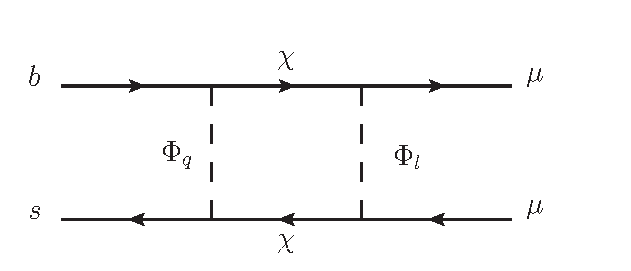
\includegraphics[width=\textwidth]{pics/bsmumu}
% \end{frame}
% \begin{frame}
% \frametitle{Flavour Anomalies}
% \setcounter{framenumber}{3}
%   \includegraphics[width=\textwidth]{pics/mumix}
% \end{frame}
\begin{frame}
\frametitle{Flavour Anomalies}
\setcounter{framenumber}{3}
  \includegraphics[width=\textwidth]{pics/all.png}
\end{frame}
\begin{frame}
\frametitle{Flavour Anomalies}

 \setcounter{framenumber}{3}
  \includegraphics[width=\textwidth]{pics/flavour.png}
\end{frame}

\begin{frame}
\frametitle{Dark Matter}
 \begin{flushright}
  \textcolor{magenta}{\tiny{Bertone' 0404175, Begemann '91, WMAP '12}}
 \end{flushright}
\setcounter{framenumber}{3}
  \includegraphics[width=\textwidth]{pics/dm.jpg}
\end{frame}
\begin{frame}
\frametitle{Dark Matter}
 \begin{flushright}
  \textcolor{magenta}{\tiny{Bertone' 0404175, Begemann '91, WMAP '12}}
 \end{flushright}
\setcounter{framenumber}{3}
  \includegraphics[width=\textwidth]{pics/dmTOT.jpg}
\end{frame}

\begin{frame}
 \frametitle{Conjecture}
 Dark matter might play the role of new particles solving the flavour anomalies
\end{frame}



\section{Model Outline}
% \begin{frame}
%  \frametitle{Basis}
% 
% Two new scalars, $\Phi_l$ and coloured $\Phi_q$, and a new fermion $\chi$ are introduced.
% 
% 
% $SU(2)_L$-irreps assigned so that
% \begin{itemize}
%  \item $L$ and $B$ violating processes prohibited,
% %  \item Coulored scalar $\Phi_q$ has weaker bounds than coulored fermion
%  \item Higgs-Pheno not modified by trilinear or quartic interactions,
% %  \item $U(1)_\chi$: FV NP loop suppressed and stable neutral $\chi$-comp.
%  \item an electrically neutral $\chi$-component exists,
%  \item dimension smaller than 5.
% \end{itemize}
%   \begin{flushright}
%   \textcolor{magenta}{\tiny{Gripaios' 1509.05020}}
%  \end{flushright}
% \end{frame}
% 
% \begin{frame}
%  \frametitle{Basis}
%  Remaining $SU(2)_L$ irrep-dimensions are triplet scalars and quadruplet fermion. Other configurations contradict assignment rules\\
%  This setup
%  \begin{itemize}
%  \item[$\checked$] is renormalisable,
%  \item[$\checked$] explains flavour anomalies,
%  \item[$\upchi$] offers no viable DM candidate.
%  \end{itemize}
% \end{frame}

\begin{frame}
 \frametitle{Basis Model}
 \visible<2->{Two new scalars, $\Phi_l$ and coloured $\Phi_q$, and a new fermion $\chi$ are introduced.\\
 Assignment rules ($L/B$-conservation, Higgs-Pheno, neutral $\chi$, minimality) only leave triplet scalars and quadruplet fermion configuration.}\\
  \visible<3->{This setup
 \begin{itemize}
 \item[$\checked$] is renormalisable,
 \item[$\checked$] explains flavour anomalies,
 \item[$\upchi$] offers no viable DM candidate $\chi^0$.
 \end{itemize}}
   \visible<2->{\begin{flushright}
  \textcolor{magenta}{\tiny{Gripaios' 1509.05020}}
 \end{flushright}}
\end{frame}

\begin{frame}
 \frametitle{Modified Model}
 \visible<2->{High $\chi$ hypercharge leads to large $Z$-coupling ($\rightarrow$ excluded by direct detection experiments).\\
 $\chi(1,1,0)$ and $\chi(1,3,0)$ with doublet (quadruplet) scalars are forbidden by $L$-conservation ($\rightarrow$ add new groups).}\\
 \visible<3->{This setup
 \begin{itemize}
  \item[$\checked$] yields a so far not excluded DM candidate,
  \item[$\checked$] also explains flavour anomalies,
  \item[$\upchi$] is not renormalisable anymore.
 \end{itemize} }
\end{frame}

\begin{frame}
\frametitle{Charge Assignment}
 \visible<2->{\begin{table}[t]
%  \resizebox{\textwidth}{!}{%
\small
 \begin{tabular}{c|c|c|c}
%$SU(3)_C\times SU(2)_L\times U(1)_{Y_W}$
  Field & $\mathcal{G}_\text{SM}$ & $A_4 \times U(1)_\text{FN} \times Z_3$ & $U(1)^3_{B,L,\chi}$\\
  \hline
  $Q^i_L$ & (3,2,$\sfrac16$) & (1,$\Upsilon_{Q_i}$,$\omega$) & ($\sfrac13$,0,0)\\
  $U^i_R$ & (3,1,$\sfrac23$) & (1,$\Upsilon_{U_i}$,$\omega^2$)& ($\sfrac13$,0,0)\\
  $D^i_R$ & (3,1,$-\sfrac13$) & (1,$\Upsilon_{D_i}$,$\omega^2$)& ($\sfrac13$,0,0)\\
  $L^i_L$ & (1,2,$-\sfrac12$) & (3,0,$\omega$)& (0,1,0)\\
  $E^i_R$ & (1,1,$-1$) & ($1 {^(} {'} {^,} '' {^)} $,$\Upsilon_{E_i}$,$\omega^2$)& (0,1,0)\\
  $H$ & (1,2,$\sfrac12$) & (1,0,1)& (0,0,0)\\
  \hline
  $\chi$ & (1,1,0) & (1,0,$\omega$)& (0,0,1)\\ %bar chi has omega**2 (?) ->Z3invariance
 & (1,3,0) & (1,0,$\omega$)&(0,0,1)\\
  $\Phi_l$ & (1,2,$\sfrac12$) & ($1''$,0,1)& (0,-1,1)\\
  & (1,4,$\sfrac12$) & ($1''$,0,1)& (0,-1,1)\\
  $\Phi_q$ & (3,2,-$\sfrac16$) & ($1$,0,1)& ($-\sfrac13$,0,1)\\
%   \hline
%   $\Phi_T$ & (1,1,0) & ($3$,0,1)& (0,0,0)\\
%   $\theta$ & (1,1,0) & (1,-1,0) & (0,0,0)
 \end{tabular}
% \caption{Transformation rules for the SM and BSM fields. $i=1,2,3$ denotes a family index. The two rows for $\chi$ denote a singlet and a triplet, respectively. For the charges under 
% $U(1)_\text{FN}$ and the representations of $E_R$ under $A_4$ see \eqref{eq_fnchargesQ} and table \ref{tab_a4charges}.}
% \label{tab_models}
\end{table}
\begin{align*}
\mathcal{L} = g_i^q \bar\chi_R Q_L^i \Phi_q + g_i^l \bar\chi_R L_L^i \Phi_l + \text{h.c.} 
\end{align*}
   \begin{flushright}
  \textcolor{magenta}{\tiny{Altarelli' 1205.5133}}
 \end{flushright}}
\end{frame}


% 
% \begin{frame}
%  self-explanatory with emphasis to 342 config 
% \begin{align}
% \mathcal{L} = g_i^q \bar\chi_R Q_L^i \Phi_q + g_i^l \bar\chi_R L_L^i \Phi_l + \text{h.c.} 
% \end{align}
% \end{frame}

\section{Phenomenological Analysis}
\begin{frame}
 \frametitle{Remarks}
 \visible<2->{\begin{itemize}
  \item Heavy scalars develop vevs triggering SSB of $A_4$ and $U(1)_\text{FN}$ and enter the couplings so that $g_2^q\approx0.04$ and $g_3^q\approx1$.
  \item $g_2^l$ shall still be variable.
  \item With this assignment $\chi^0$ might be Majorana.
  \item Considered isospin configurations for the NP fields $(\chi,\Phi_l,\Phi_q)$ are (1,2,2), (3,2,2) and (3,4,2).
  \item Introduce $x_{q,l} = \frac{M_{q,l}^2}{m_\psi^2}$
 \end{itemize}}
 \end{frame}

 \begin{frame}
  \frametitle{Semileptonic Decay}
  \begin{minipage}{0.6\textwidth}
\visible<2->{  In configuration (122) no charged currents possible $\rightarrow$ no $O_{lq}^{(3)}$. Box (a) yields
  \small
\begin{align*}
  \mathcal{L}^{{122}}_\text{eff} \supset \frac{K(x_q,x_l)}{m_\chi^2}\frac{g_i^{q*} g_j^{q*} g_m^l g_n^l}{64\pi^2}  \left(O_{lq}^{(1)} + 0\, O_{lq}^{(3)}\right).
\end{align*}}
\normalsize
\visible<3->{Relative operator coefficient depends on tensor product decomposition of irreps:
\small
\begin{align*}
 \mathcal{L}^{{322}}_\text{eff} \supset \frac{K(x_q,x_l)}{m_\chi^2}\frac{g_i^{q*} g_j^{q*} g_m^l g_n^l}{64\pi^2}\left(O_{lq}^{(1)} + \frac23 O_{lq}^{(3)}\right),
 \end{align*}
    \begin{align*}
 \mathcal{L}^{{342}}_\text{eff} \supset \frac{K(x_q,x_l)}{m_\chi^2}\frac{g_i^{q*} g_j^{q*} g_m^l g_n^l}{64\pi^2}\left(O_{lq}^{(1)} - \frac13 O_{lq}^{(3)}\right).
 \end{align*}}


  \end{minipage}
  \begin{minipage}{0.2\textwidth}
  \visible<2->{ 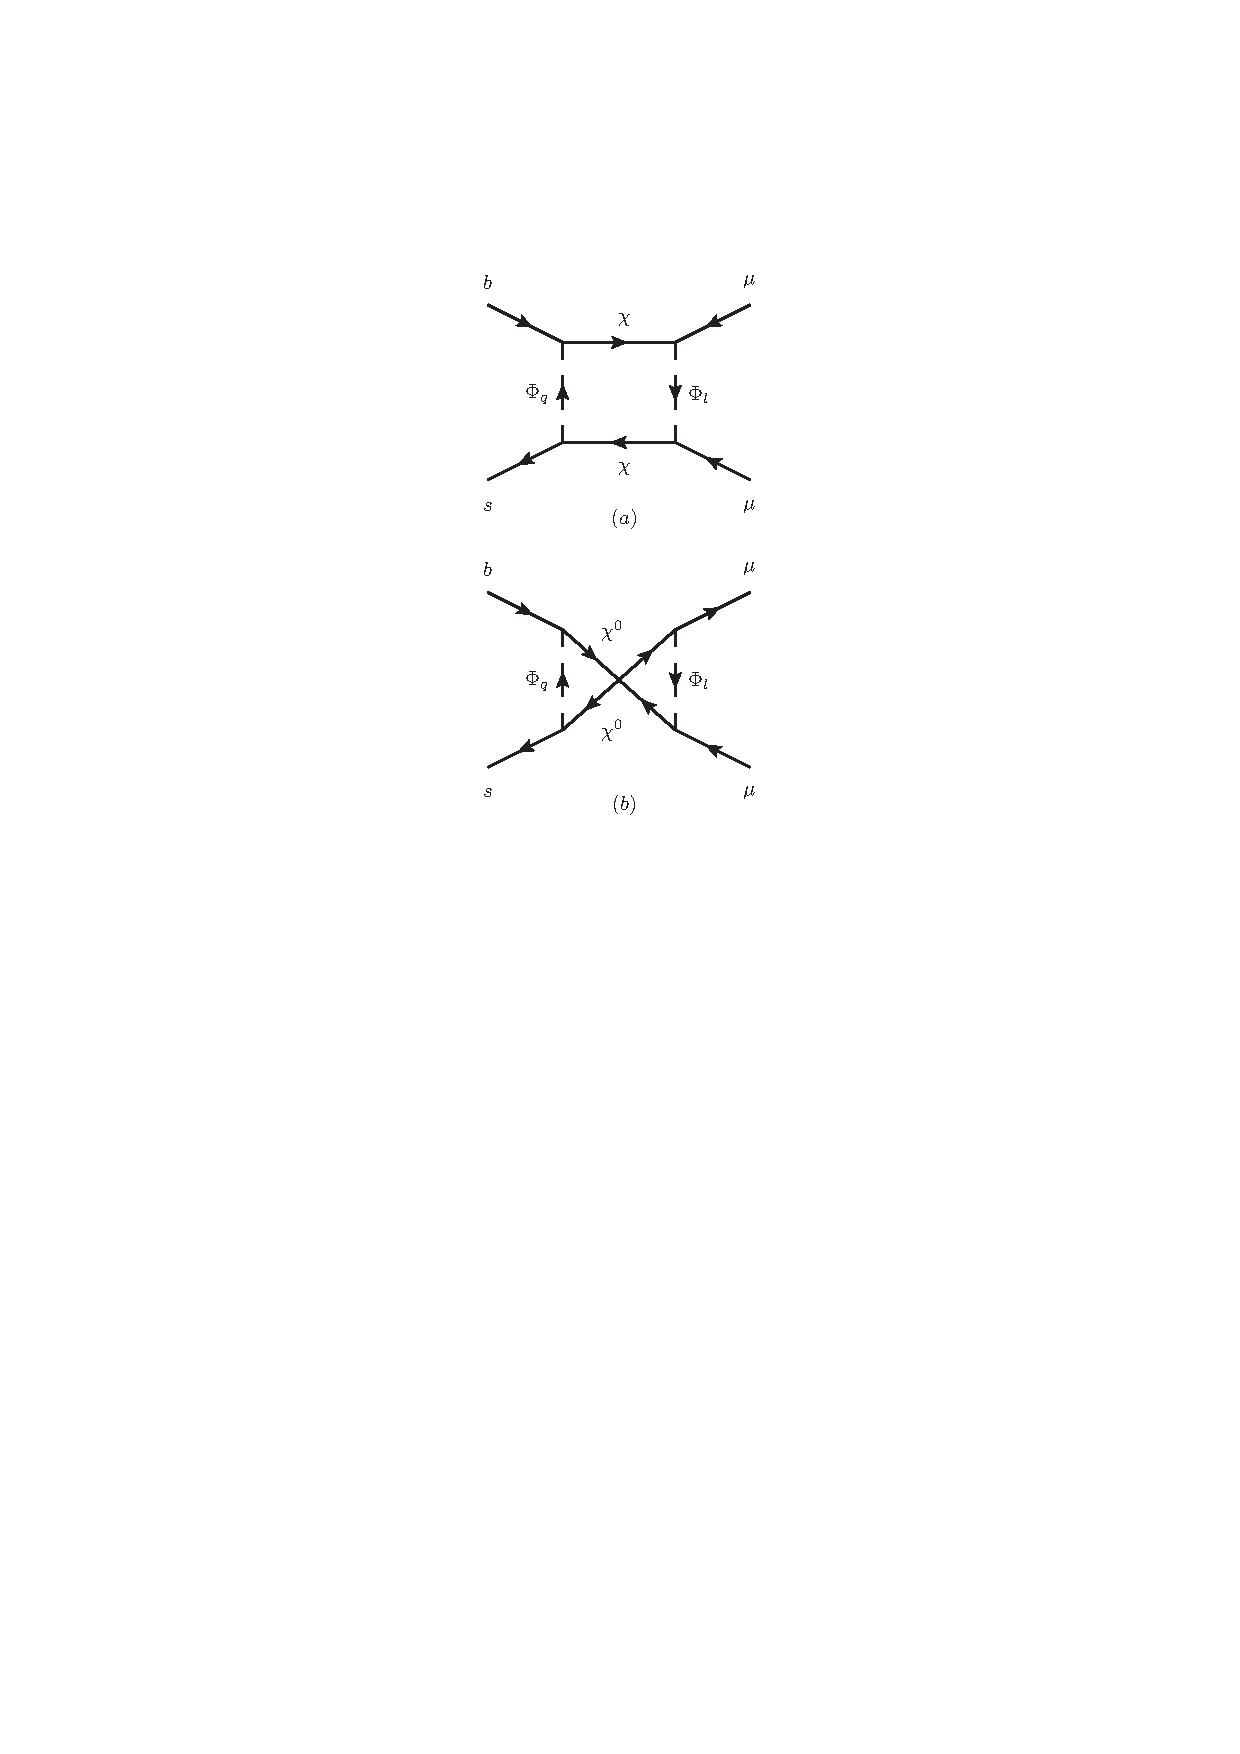
\includegraphics[width=1.9\textwidth]{pics/bsmumuVert.pdf}}
  \end{minipage}
       \visible<2->{ \begin{flushright}
  \textcolor{magenta}{\tiny{Grzadkowski' 1205.5133, Altmannshofer' 1411.6743}}
 \end{flushright}}

 \end{frame}

 \begin{frame}
 \frametitle{Semileptonic Decay}
 \normalsize
Crossed box (b) only possible with Majorana $\chi^0$. Wilson coefficients of concerned effective operators $O_9$ and $O_{10}$ for $b\rightarrow s\mu\mu$
 transitions receive contibution ($C_9 = -C_{10} \approx -0.7$):
 \small
 \begin{align*}
   C_9^{122} &\sim  \frac{g_2^{q*}g_3^q|g_2^l|^2}{m_\chi^2} \frac{1}{128\pi^2} \left(K(x_q,x_l) + 2G(x_q,x_l)\right)\label{eq_WilsonBsmumu122}\\
 C_9^{{322}} &\sim  \frac{g_2^{q*}g_3^q|g_2^l|^2}{m_\chi^2} \frac{5}{384\pi^2} \left(K(x_q,x_l) + 2\cdot\frac15 G(x_q,x_l)\right)\\
 C_9^{{342}} &\sim  \frac{g_2^{q*}g_3^q|g_2^l|^2}{m_\chi^2} \frac{1}{192\pi^2} \left(K(x_q,x_l) + 2\cdot\frac13 G(x_q,x_l)\right)
 \end{align*}
 \normalsize
Note: $\gamma/Z$-penguin contribution at \% level.
 
         \begin{flushright}
  \textcolor{magenta}{\tiny{Altmannshofer' 1411.3161, Hiller' 1408.1627, Arnan' 1608.07832}}
 \end{flushright}
 \end{frame}

 \begin{frame}
  \frametitle{Meson Mixing}
    \begin{minipage}{0.6\textwidth}
\visible<2->{Similarly for $B_s \bar B_s$-mixing for $O_{B \bar B}$:
    \small
   \begin{align*}
  C_{B\bar B}^1 &=  \frac{|g_2^{q*}g_3^q|^2}{m_\chi^2} \frac{1}{128\pi^2} \left(K'(x_q) + 2 G'(x_q)\right),\\
 C_{B\bar B}^3 &=  \frac{|g_2^{q*}g_3^q|^2}{m_\chi^2} \frac{5}{384\pi^2} \left(K'(x_q) + 2\cdot\frac15 G'(x_q)\right).
\end{align*}
\normalsize
Positive for $x_q>1$.}\visible<3->{ But constraint is strong
\begin{align*}
 C_{B\bar B} \in [-2.1,0.6] \times 10^{-5} \text{TeV}^{-2} \quad(2\sigma)\,.
\end{align*}
$K'(x)$ and $G'(x)$ may cancel each other out.}

  \end{minipage}
  \visible<2->{\begin{minipage}{0.2\textwidth}
   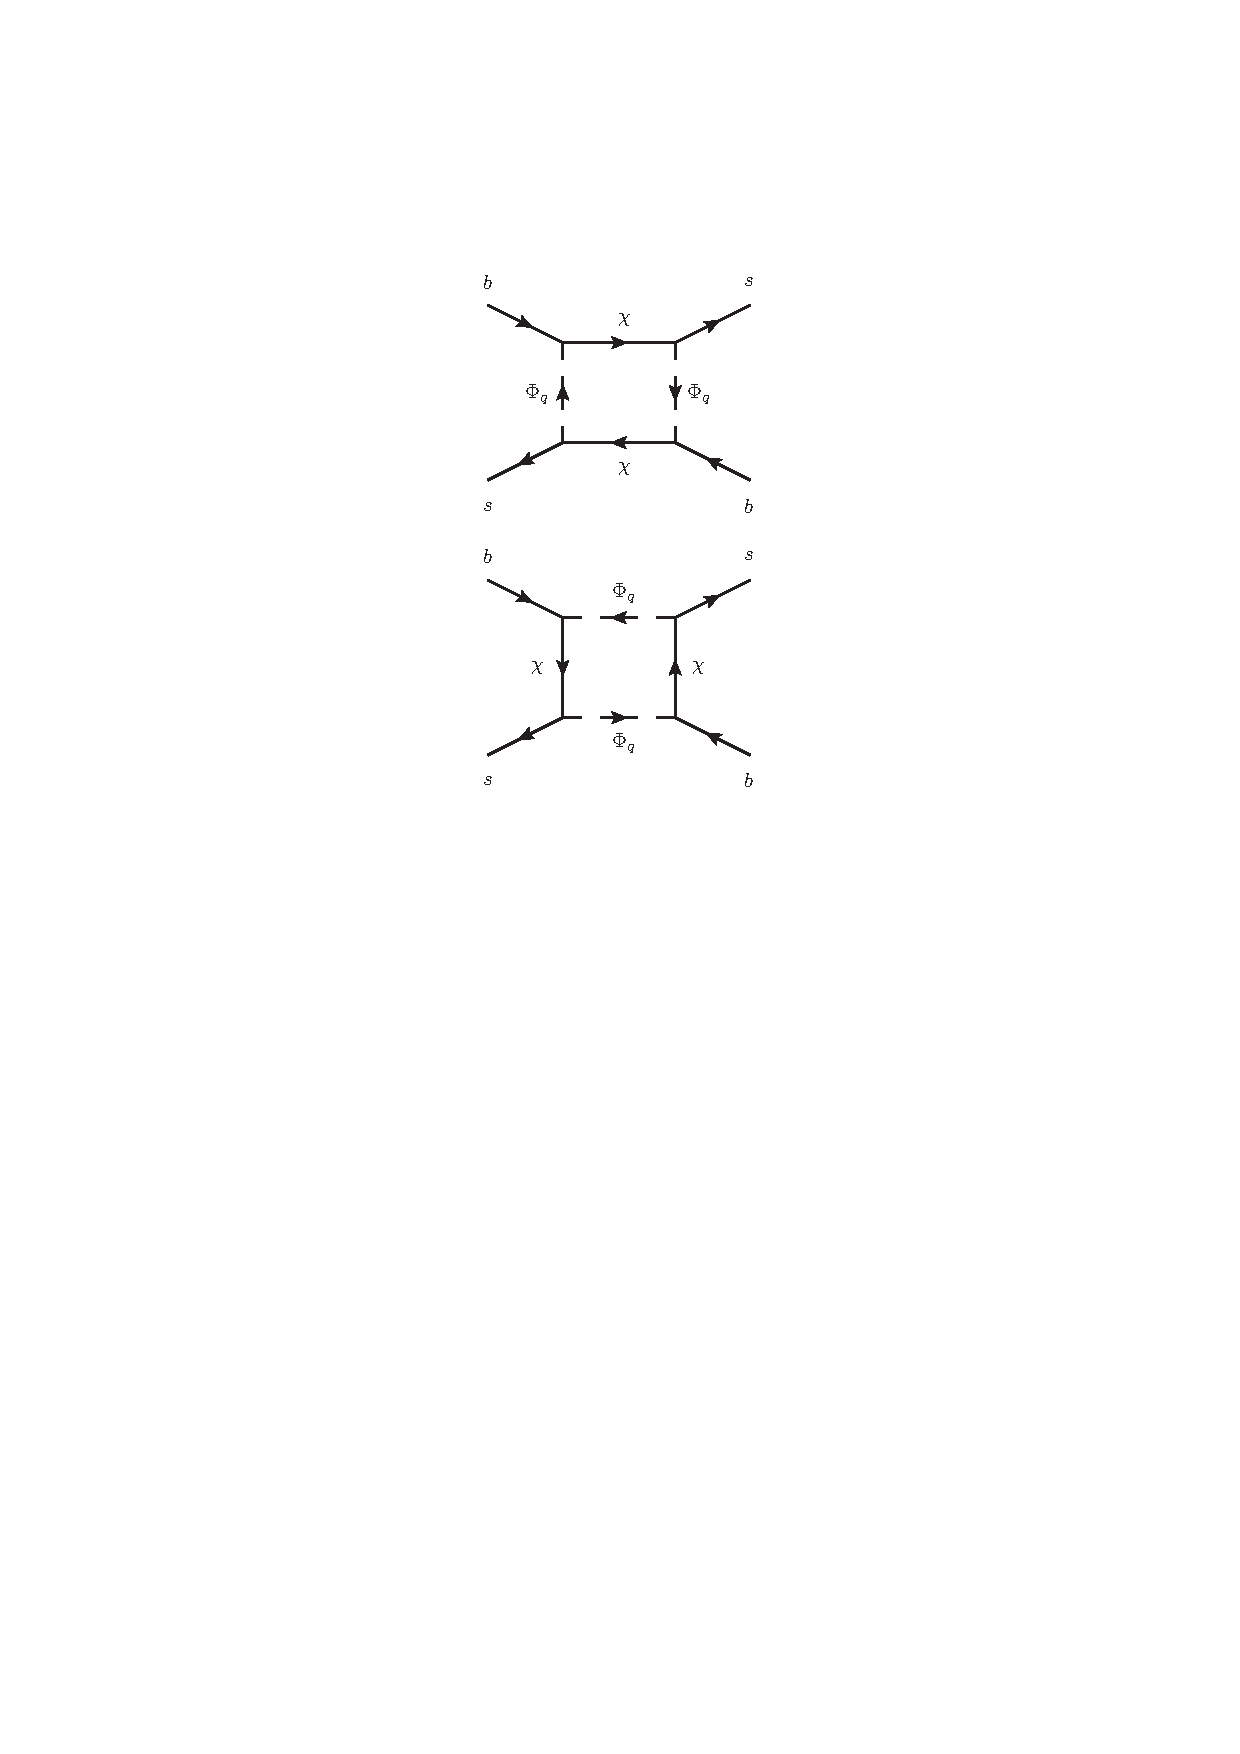
\includegraphics[width=1.9\textwidth]{pics/bsmixVert.pdf}
  \end{minipage}
        \begin{flushright}
  \textcolor{magenta}{\tiny{MILC' 1602.03560}}
 \end{flushright}}
 \end{frame}

 \begin{frame}
  \frametitle{Anomalous Magnetic Moment of the Muon}
  \visible<2->{Basis model states that SM deviation is large ($\approx 3\times10^{-9}$). NP contribution:
  \begin{align*}
   \Delta a_\mu=\frac{|g^l_2|^2}{16\pi^2} \frac{m^2_\mu}{m_\chi^2}\left(Q_\chi^i I(x_l) + Q_{\Phi_l}^i \frac{1}{x_l} I(x_l^{-1}) \right)
  \end{align*}}
  \visible<3->{Summed up charges (1st line: basis model):
  \begin{align*}
 Q_\chi &= 5,\,Q_{\Phi_l} = 3 \qquad \text{(433)},\\
 Q_\chi &= 0,\,Q_{\Phi_l} = 1 \qquad \text{(122)},\\
 Q_\chi &= 1,\,Q_{\Phi_l} = 1 \qquad \text{(322)},\\
 Q_\chi &= 0,\,Q_{\Phi_l} = 3 \qquad \text{(342)}.
\end{align*}
  $\frac{1}{x_l} I(x_l^{-1})$ term has larger impact. So, high $Q_{\Phi_l}$ needed.}
          \visible<2->{\begin{flushright}
  \textcolor{magenta}{\tiny{Lavoura' 030222, Muon g-2' 0602035}}
 \end{flushright}}
 \end{frame}

 

\begin{frame}
\frametitle{Dark Matter Phenomenology}
\visible<2->{Assume $\chi^0$ to be thermally produced. Relic density
\begin{align*}
 \Omega_\text{DM} h^2 \approx 0.11805 \approx \frac{10^{-26} \text{cm}^3 / \text{s}}{ \langle \sigma v \rangle_\text{Ann}}.
\end{align*}
Annihilation mostly into muons, $W$-bosons, tops. Dirac DM annihilation leaves a too small $\Omega_\text{DM}$.}\\
\visible<3->{SD direct detection below bounds by 4 orders of magnitude. }\\
\visible<4->{Singlet case: SI form factor suppressed by $M_{\Phi_q}^4$. Cross section below by 2 orders of magnitude.\\
Triplet case: $m_\chi$ is sole model parameter. Examined by XENON1T this year. }
          
         \visible<2->{ \begin{flushright}
  \textcolor{magenta}{\tiny{Planck' 1303.5076, Bruggisser' 1607.02475, IceCube' 1212.4097, Hisano' 1104.0228, XENON' 1512.07501}}
 \end{flushright}}
\end{frame}

\section{Results}
\begin{frame}
 \frametitle{Scalar masses}
 \visible<2->{SM-charges of NP fields make them look like SUSY-particles: Bino/Wino $\chi$, smuon $\Phi_l$, sbottom $\Phi_q$.\\
 But couplings are not SUSY-like.}
 \visible<3->{We consider $m_\chi < M_l < M_q$ (stable DM, maximal $(g-2)$, minimal $B$-mixing) and take $M_l\gtrsim300$\,GeV, $M_q\gtrsim720$\,GeV.}
\visible<2->{            \begin{flushright}
  \textcolor{magenta}{\tiny{ATLAS' 1506.08616}}
 \end{flushright}}
\end{frame}

\begin{frame}
 \frametitle{$C_9$ for Different Configurations}
 \visible<2->{\centering
 \includegraphics[width=0.7\textwidth]{pics/BsmumuReps.pdf}\\
 \flushleft
 Contour plot for bounds of $b\rightarrow s \mu\mu$ for different configurations. Lines denote upper boundaries of one standard deviation. Lower
 ones lie above but are not shown.}
\end{frame}

\begin{frame}
 \frametitle{Impact of $G'(x_q)$ on Meson-Mixing}
 \visible<2->{ \centering
 \includegraphics[width=0.7\textwidth]{pics/fa23BBReps.pdf}\\
 \flushleft
 Upper bounds of $B_s$-mixing for singlet and triplet $\chi$. ``M'' is considering $\chi^0$ Majorana, ``D'' Dirac. 
 Regions each below are allowed. Purple line is our expectation.}
\end{frame}

\begin{frame}
  \frametitle{DM Mass for (122)}
  \visible<2->{\centering
 \includegraphics[width=0.6\textwidth]{pics/contour122.pdf}\\
 \flushleft
 Singlet DM only gets constraints from annihilation and $b\rightarrow s\mu\mu$. $\Delta a_\mu$ contribution $\approx20\,\%$. Good solutions on blue solid line. }
\end{frame}

\begin{frame}
  \frametitle{DM Mass for (322)}
  \visible<2->{\centering
 \includegraphics[width=0.6\textwidth]{pics/contour322.pdf}\\
 \flushleft
 Additional constraint from Meson-mixing. Slight increasing of $M_q$ reduces this influence without changing other processes too much. 
 $\Delta a_\mu$ contribution $\approx50\,\%$.}
\end{frame}

\begin{frame}
  \frametitle{DM Mass for (342)}
  \visible<2->{\centering
 \includegraphics[width=0.6\textwidth]{pics/contour342-770.pdf}\\
 \flushleft
 $M_q$ set to 770\,GeV. All processes can be explained. Luckily, $C_9$ and $\Delta a_\mu$ both need high $g^l_2$. }
\end{frame}


\begin{frame}
 \frametitle{Conclusion}
 \small
 \visible<2->{Problem: Basis model has no viable DM candidate.\\
 \begin{itemize}
  \item Enabling afore forbidden irreps by adding $A_4$.
  \item Explaining fermion mass hierarchy and estimating new couplings with $U(1)_\text{FN}$.
 \end{itemize}}
 \visible<3->{Isospin singlet/triplet NP fermion contains possible Majorana DM candidate.
\begin{itemize}
 \item Neither one is currently exluded by direct detection.
 \item (342) configuration can explain all flavour processes and yields correct RD
\end{itemize}}
\visible<4->{Tradeoff: loss of renormalisability.}

\end{frame}

\begin{frame}
\centering
 Thank you for your attention!
\end{frame}



 





\end{document}
